\documentclass[11pt]{article}

\usepackage{fullpage}
\usepackage{tikz}
\usepackage{listings}
\usetikzlibrary{shapes,arrows}

\begin{document}

\title{Group 6 Final Report}
\author{Chan Chun ckc116, Cheung Ka hlc116, Mang Hao hxm16, Cheuk Ki kfc216}

\maketitle

\section{Implementation of the assembler}

 
After careful discussion, we have decided to implement the assembler using two passes over the source code as specified in the spec, which then leads to the following structure:\newline\newline
Structures:
Linkedlist,
BST,
Line tokens,
Instructions
\newline
Tokenizer
(tokenizer.c)
(tokenizer.h)\newline
Table
(table.c)
(ADT{\_}BST.c)
(ADT{\_}linkedlist.c)\newline
I/O
(assemble.c)\newline
Assembing instructions
(ass{\_}branch.c)
(ass{\_}dp.c)
(ass{\_}multiply.c)
(ass{\_}sdt.c)\newline
Two-pass assembly
(firstpass.c)
(secondpass.c)\newline
Utility function
(ass{\_}util.c)\newline
Main
(assemble.c)

\subsection{Reading the source file}
\begin{itemize}  
\item Use the function sourcefilereader()  in ass{\_}util.c

\item Store the number of lines for further uses 

\item Store the content of the source file in an array of char*[100] for further use, assuming that the number of lines will not exceed 100  

\end{itemize}





\subsection{Parsing the file}
\begin{itemize}  
\item Use the function filetotokens() in tokenizer.c
\item Each line is stored in a struct showed beside
\item Type include label and operands, line{\_}token with type operands will have the opcode enable and vise versa
\end{itemize}


\subsection{First pass}
Extracting all lines which has the type of LABEL and create a table, using a LINKEDLIST structure implemented by us, each element is stored with the name of the label and the index (the relative position of the label in the instructions)
\subsection{Calling appropriate functions depending on the opcode (Second Pass)}
By using an if else branch, separate different LINE{\_}TOKENS according to their opcode (e.g. MOV, STR, LDR, etc..), call the appropriate functions and providing other information to the functions if required . This functions called are expected to return a type of following struct: 

\begin{center}
\begin{tabular}{|c|c|}
\hline
\begin{lstlisting}[language = C]
typedef struct {
   char type[20];
   union {
	DATAPROCESSING_INSTR *dp; 
	MULTIPLY_INSTR *mp;
	SIN_DATA_TRAN_INSTR *sdt;
	BRANCH_INSTR *br;
   } instr;  
} INSTRUCTION;
\end{lstlisting} &

\begin{lstlisting}[language = C]
typedef struct br {
   u32 INSTRUCTION;
   char OPCODE[4];
   u32 COND: 4;
   u32 OFFSET;
} BRANCH_INSTR;
\end{lstlisting}\\
\hline

\end{tabular}
\end{center}

\subsubsection{Data Processing}
The only part worth mentioning is the part identifying different types of operand2 , this is achieve by using several if else, which include figuring the first character of the operand is a '\#' or not to seperate shift register and expression, and also the number of operands in LINE{\_}TOKEN to figure out is there a shift or not

\subsubsection{Branch}
\begin{itemize}  
\item Additional information: linked list which stores the labels, the address of the current line

\item It first look up the address of the label by looking up the linked list, calculate the offset by considering the current address and also the pipeline principle.

\item It then transform the offset,which is in type INT into two complements using a helper function transformnum(), the two complements are stored as u32 (unsigned 32 bit).
\end{itemize}




\subsubsection{Single Data Transfer}
\begin{itemize}  
\item Additional information: address of current line, the number of total instructions (to determine the offset when loading an expression)

\item Parts for calculating the offset with immediate value and also shifting register are approximately the same as the parts in Data Processing, but with few more exceptions

\item Instead of using if else loop to identify different type of <address>, a helper function parseExpressioninrect() is used, which identify different types by calculating the number of expressions in square bracket and the number of exp not in bracket
\end{itemize}

\subsubsection{Multiply}
This part is pretty straight forward, just need to fit in different register to appropriate field in INSTRUCTION.

\subsection{Assemble the INSTRUCTION into binary (Second Pass)}
This is achieved by simply shifting to the appropriate position. E.g. instruction. A tiny remark is that we realise using |= rather than += will be easier for debugging. If we use +=, if the field (e.g. DEST in DATAPROCESSING{\_}INSTR) is longer than its expected length, it will create a mess and super difficult to debug, especially when its a binary code. So we changed to |= later on. |= and += has the same effect if all of the field has appropriate length and is not overlapping, which in fact, they should not be overlapping.



\section{Description of our extension - Simon}
Our extension is to implement an early version of the game Simon -- a simple game which trains the memorisation of children. In our game, there are 4 buttons which correspond to the 4 LEDs of different colours for the player to press on. In each round a sequence of LEDs would light up, the player then have to repeat the sequence by pressing the buttons corresponding to each LED. The next element of the sequence is randomly generated by a random generator and will be stored for use in the entire game. The game is made harder and harder by adding one more element to the sequence in each consecutive round. In our game, there are two levels which consists of sixteen rounds each. The second level is more difficult as we reduce the delay between the lights on of the LEDs in a sequence. Below are the layout of the game:
\begin{figure}[h!]
\centering
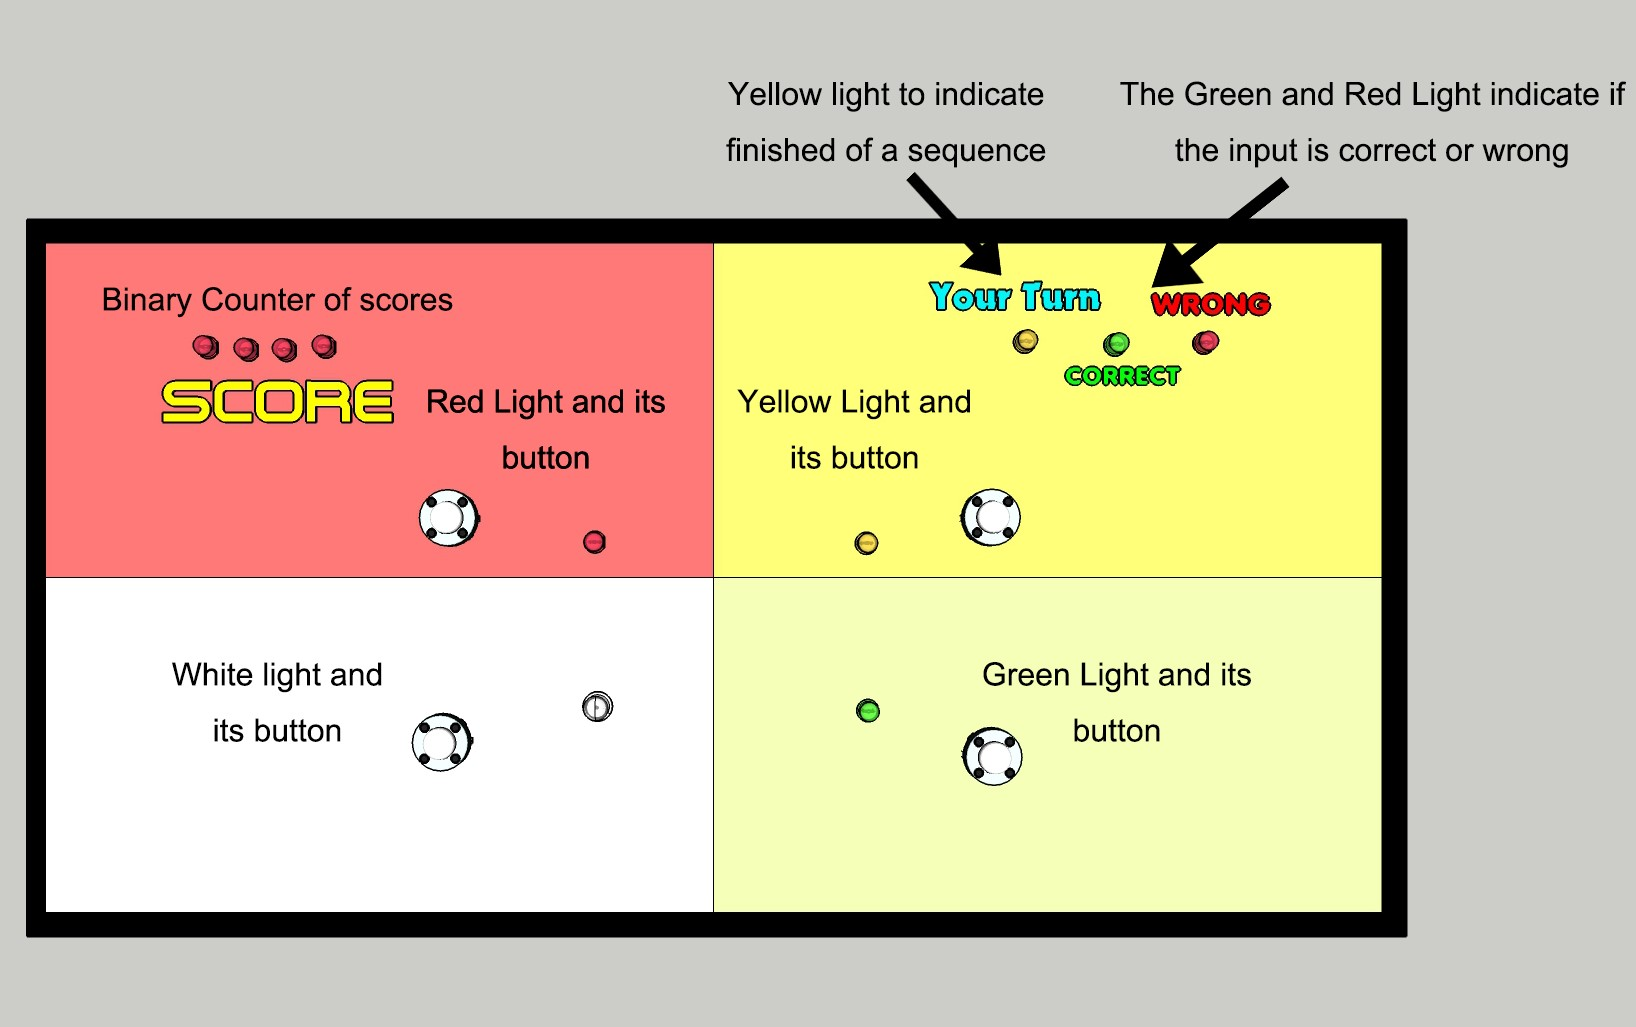
\includegraphics[width = 0.75\linewidth]{TOP1.jpg}
\caption{Layout of the game}
\label{fig::layout}
\end{figure}

We used C to program the game $(./arm11{\_}06/extension/simon.c)$ and library bcm2835 to access the GPIO pins of Raspberry Pi (Revision 2). Each pin are corresponding to one LED or button. As figure \ref{fig::layout} shows, there is a binary counter to calculate the score of the player, three state indicating lights (Yellow, Green and Red)to represent finishing of a sequence, correct input and wrong input respectively. Below are the flowchart of the game.

%Flow Chart for games
% Define block styles
\tikzstyle{decision} = [diamond, draw, fill=blue!20,
   text width=4.5em, text badly centered, node distance=3cm, inner sep=0pt]
\tikzstyle{block} = [rectangle, draw, fill=blue!10,
   text width=15em, text centered, rounded corners, minimum height=4em]
\tikzstyle{line} = [draw, -latex']
\tikzstyle{blocks} = [rectangle, draw, fill=blue!10,
   text width=5em, text centered, rounded corners, minimum height=4em]
 
 \begin{tikzpicture}[node distance = 2cm, auto]
 
   % Place nodes
   \node [block] (start) {Start The game at level 0};
   \node [block, below of=start] (random) {A random sequence is generated followed by yellow light on the top right corner blinking};
   \node [decision, below of=random] (input) {Correct Input?};
   \node [block, right of=input, node distance=5cm] (correct) {Correct sequence , the green light on the top right corner will blink to indicate correct};
   \node [block, left of=input, node distance=5cm] (wrong) {The red light on the top right corner will blink to indicate wrong input.};
   \node [block, below of=correct, node distance=2cm] (counter) {The binary counter of score will increment by 1 and each 16 score will increase 1 level};
   \node [block, below of=counter, node distance=2cm] (win) {Once the player finished level 2, the player win the game};
   \node [blocks, right of=random, node distance=8.5cm] (wait) {Prints winning pattern};
  
   % Draw edges
   \path [line] (start) -- (random);
   \path [line] (random) -- (input);
   \path [line] (input) -| node [near start] {no} (wrong);
   \path [line] (input) -- node  {yes} (correct);
   \path [line] (correct) -- (counter);
   \path [line] (correct) |- node[near start]{wait for next sequence}(random);
   \path [line] (wrong) |- node[near start]{restart}(start);
   \path [line] (counter) -- (win);
   \path [line] (win) -| (wait);
   \path [line] (wait) |- node[near start]{restart}(start);
 
\end{tikzpicture}
\begin{figure}[h!]
\caption{Flow chart of the game}
\end{figure}


\section{Design and the associated challenges of Simon}
During the extension implementation, there are two main problems.
\begin{itemize}
\item Hardware problems, as most of our team members are not familiar with electronic, we are confused on connecting wires on the breadboard and often encounter bugs caused by hardware problems (The LED is not blinking and no valid input is taken because of wrong circuit design)
\item Software problems, as we are using a library bcm2835, many of its functions are unfamiliar to us and sometimes we may misunderstood the function.
\end{itemize}

\section{Testing for our implementation on Simon}

Simon’s say is not a super complicated game, but still it require some testing in order to make the game run smoothly.\newline\newline
Testings are not done only when the whole program is implemented. Instead, testings are carried out for each functions when they are implemented. For example, we test the game algorithm (simon.c) in the ide console before implementing it with the raspberry pi.\newline \newline
When debugging the functions, we have design a few general test cases and then input the variables manually. Then some group mates carry on implementing other functions while others will continue testing the function by designing more specific edge cases.\newline \newline
We have used the library bcm2835.h in order to access different pins. Before using the library in our program, we have tested the library with some simple functions to make sure that the library works and we understand the properties of functions from the library. We have that each pin can be set as input and output, output pin can be set and clear properly etc.. before implementing the game with the raspberry.\newline \newline
It is also important for us to test each hardware components. We have to make sure that they are all working properly before the final tests. If we don't do this, we won't know whether it is a hardware failure or a software bug during the final debug, and will cause additional work in order to identify it. Therefore we have made sure that all parts are working, and the circuits are connected correctly before debugging the game.\newline \newline
We test the program in this way due to the lessons learnt when debugging assembler, While debugging assembler, it is really time consuming and difficult to debug the program as a whole. Therefore when working on the extension, we test while we are coding.\newline \newline
After making sure that each functions works, we can move on to a larger scale of testing. Simon’s says is not very complicated and the gameplay is rather straightforward, therefore we have played the game for a number of times in order to make sure that the game works in general.\newline 
Later on, we have discussed and design a few edge cases for testing. Which includes intentionally pressing the wrong button at the wrong time, or winning the games for too many times. One remark on the later cases is that, as testing this case by winning the games are time consuming and inefficient. We have changed and implement the code in such a way that we can manually change the variable and make the program thinks that we have already won a lot of levels. We learnt that in the sense of debugging, it is usually more convenient to debug of we make some variables easy to change, though this may cause is the security problem in other situations, it is not our concern for this game.


\section{Group Reflection}
In the beginning of the project, we mainly work together as a group in the lab with some team members programming while others do research. Working in this way helps us resolve any problem very quickly as we can support each other face-to-face. Also, we found this beneficial because we are not familiar with C in the very beginning and lots of help is needed. However, working together in the lab means that we will have to work on each part of the project one at a time, which slows down the progress. Since we all know more about C in the middle of the project and require less support from each other, we changed our approach when working on the assembler. This is the moment when we divide work amongst all members to allow work being done individually, each member is responsible for several branches on git which we later merge them into a single file. The efficiency has since then increased a lot. If we were given the chance to start the project again, we would have started work allocation straight from the start of the project so that members can do their own individual research back at home and discuss about problems and difficulties when we are having our team meeting. In conclusion, we are satisfied on our work allocation and team communication and are looking forward to collaborate in the future.

\section{Individual Reflection}
\textbf{Hao, Mang (hxm16):}
\\ Across the project, I found it satisfying and demanding. My WebPA feedback proven I am active member of the team and making a great contributions throughout the whole project.
\\When I first start off, I felt very uncomfortable in the team  as I didn’t know well about the strength of my teammates, so it is hard to coordinate the team to work efficiently in the beginning. Also, as we are unfamiliar with Git and C programming, many of our works are having conflicts. So, in the first two week, we are behind schedule. I feel our group time management could have been improved if we have a better communication in the team. It will save a lot of time for explain the specification to the teammate who are behind progress.
\\In the future projects, I will maintain the skills of setting deadlines and milestones at the beginning of the project. It have been proven to be a effective ways to improve our time management in the project.
\\
\\
\textbf{Ka, Cheung (klc116):}
\\
\\
\textbf{Ki, Cheuk (kfc216):}
\\Throughout the project, i realise that debugging is a really important process, and difficult as well if good practises are not implemented. I learnt that it is usually a beneficial  to use the function printf() and state which part the program is running, and also print out the partial processed variables so that i can check whether the code is doing what we want it to do.
\\On the other hand, it is also really important to implement a set of detailed test cases, i realised that missing edge cases may cause a huge problem later on. For example, we didn’t consider some special cases when debugging assembler. Then later on it turn out to be a problem when we are implementing the raspberry pi and the extension. It cost a lot of time for us to solve this kinds of problem. 
\\This project also teach me that communication with teammate are in fact, more important than I have thought. For example, even we have allocated our work while implementing assembler, I should have discuss with my teammates more frequently so that I will have a better understanding of how each part of the program interact with each other. Many bugs are caused by these poor understandings of each other's work.
\\
\\
\textbf{Chun, Chan (ckc116):}




\end{document}
